\section{Introduction}

\mm{Reorder a little bit such that the motivation and existing approaches to total order are introduced first and then epto is presented as an alternative approach. Also stress the motivation is to run a TO algorithm in a very large scale and draw insights from it, similarly to what was done in the papers "paxos made live" and "worldwide consensus.". Point out that there are few works evaluating such protocols in a really large scale.}\mm{We also need to make the contribution clear: In this case it is an implementation of a total order algorithm and making it available as open source. It would be good if we could put this on a more generic light, along the lines of "a set of tools to evaluate large scale algorithms" or at least present the tool itself, eptotester as a contribution, wdyt ? this would make the paper stronger }

Creating an algorithm providing scalability, integrity and validity, along with a total ordering of the events through all peers in a distributed network has been one the hot topics in distributed computing research for many years. One of the recently designed algorithms on this topic is \epto \autocite{matos2015epto}. \epto is an algorithm that claims to provide integrity, validity and total order in a large-scale distributed system. Furthermore, \epto is designed to work without a global clock, removing the need to synchronize clocks precisely on every peer and thus is well-suited for these kind of systems.
\par 
There are many other algorithms for disseminating and ordering events in a distributed network. There are deterministic algorithms, which guarantee total order, agreement or other strong properties. Unfortunately, these types of algorithms are not scalable enough to be used in large-scale distributed systems \autocites[]{defago2004total}[]{lamport1978time}.
\par
The problem with existing deterministic total ordering protocols is that they need some sort of agreement between all peers in the network. This causes a massive amount of network traffic and overhead on the system.
Moreover, an agreement feature for an asynchronous system requires to
explicitly maintain a group and have access to a failure detector \autocites[]{chandra1996weakest}[]{chandra1996unreliable}. Due to faults and churn in large-scale distributed systems, the failure detector turns into a bottleneck for the structure and thus limits the algorithm's scalability.
\par
As an alternative to deterministic algorithms, there are probabilistic algorithms, focusing on scalability and resiliency against failures using a probabilistic dissemination approach  \autocite{birman1999bimodal,carvalho2007emergent,demers1987epidemic,eugster2003lightweight,felber2002probabilistic,hayden1996probabilistic,kim2004gossip,Koldehofe02simplegossiping}. These algorithms guarantee the dissemination of events in the system with high probability. This way, there is no need for failure detectors and redundant traffic, making these algorithms highly scalable. As these algorithms focus on reliability of dissemination, they often have to ignore other properties such as total ordering.
\par
\epto claims to solve these seemingly irreconcilable differences. By using a probabilistic dissemination together with deterministic ordering, \epto provides total order along with scalability, validity and integrity. \epto consists of two distinct components. \epto's dissemination component guarantees that all peers will receive an event with arbitrarily high probability. Once peers have received all events, \epto's ordering component orders them using the events timestamp, and in case of a tie use the broadcaster ID of the events.
\par
To model the first component, \epto is using a \textit{balls-and-bins} approach \autocite{Koldehofe02simplegossiping}. The \textit{balls-and-bins} problem is a basic probabilistic problem: consider \textit{n} balls and \textit{m} bins where we consequently throw balls into a bin uniformly at random and independently from other balls. In this scenario, one of the natural questions that comes to mind is: what is the minimum number of balls that should be thrown, so that every bin has at least one ball with high probability?
\begin{figure}
	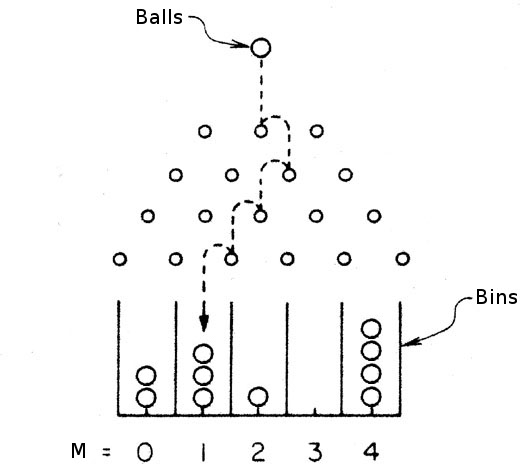
\includegraphics[width=\linewidth]{figures/BnB.jpeg}
	\caption[Caption]{Balls-and-Bins\footnotemark}
	\label{fig:balls-and-bins}
\end{figure}
\footnotetext{Figure inspired from \autocite{bnb}}
\par
Using the balls-and-bins approach we model processes as bins and events as balls and calculate how many balls need to be \textit{thrown} such that every bin contains at least one ball with arbitrarily high probability. With this approach the number of messages transmitted per process per round is logarithmic in the number of processes, therefore the number of messages sent in the system is low and uniform over all processes. Thanks to these approaches, \epto is highly resilient with  imperfect networks and highly scalable as the networks grow, while always providing total order. \par
Until now, the creators of \epto have only tested this algorithm in a simulated environment. In this work, we implement \epto in pure Kotlin\footnote{\href{https://kotlinlang.org/}{https://kotlinlang.org/}} and introduce a benchmarking solution to show that \epto is suitable for real-world large-scale distributed systems. We compare \epto to the deterministic total order algorithm provided by \jgroups \autocite{jgroups} in both stable and unstable environments. \epto uses a PSS CYCLON \autocite{Voulgaris2005} to obtain a random view. Peers use a tracker that keeps track of dead and alive peers when they first join the network. These benchmarks can easily be launched and scaled on a cluster using Docker and Docker Swarm. Furthermore, we can inject synthetic or real churn using the Failure Trace Archive databases\footnote{\href{http://fta.scem.uws.edu.au/}{http://fta.scem.uws.edu.au/}} in the system.
\par
The next sections present our benchmarking solution and the results obtained. Section \ref{sec:background} exposes the background of \eptotester and presents the different kind of ordering. Section \ref{sec:definitions} defines the terms used in the paper. Section \ref{sec:epto} presents \epto and the architecture of our implementation. Section \ref{sec:evaluation} shows and explains the results obtained as well as the limitations our project faced. We then present possible future work in Section \ref{sec:future-work}. We finally conclude in Section \ref{sec:conclusion}.
